\documentclass[
	article,
	11pt,
	twoside,
	a4paper,
	english,
	brazil,
	sumario=tradicional
	]{abntex2}

\usepackage{helvet} 
\usepackage[T1]{fontenc}		
\usepackage[utf8]{inputenc}	
\usepackage{indentfirst}
\usepackage{nomencl}
\usepackage{color}
\usepackage{graphicx}
\usepackage[export]{adjustbox}
\usepackage{microtype}
\usepackage{float}
\usepackage{pdfpages}
\usepackage{scalefnt}
\usepackage{authblk}
\usepackage{multicol}
\usepackage{amsmath}
\usepackage{wrapfig}

\linespread{1.5}

\renewcommand\Authands{ e }
\renewcommand{\familydefault}{\sfdefault}

\setlrmarginsandblock{4cm}{4cm}{*}
\setulmarginsandblock{4cm}{4cm}{*}
\checkandfixthelayout

\usepackage[brazilian,hyperpageref]{backref}	 % 
\usepackage[alf]{abntex2cite}

\renewcommand{\backrefpagesname}{Citado na(s) página(s):~}

\renewcommand{\backref}{}
\renewcommand*{\backrefalt}[4]{
	\ifcase #1 %
		Nenhuma citação no texto.%
	\or
		Citado na página #2.%
	\else
		Citado #1 vezes nas páginas #2.%
	\fi}

\titulo{Fundamentos de contagem} 
\author[*]{Ítalo Epifânio de Lima e Silva}
\author[*]{Andressa Elna Mesquita Belém}
\affil[*]{Universidade Federal do Rio Grande do Norte, UFRN}

\local{Natal, RN}
\data{2018}

\definecolor{blue}{RGB}{41,5,195}

\makeatletter
\hypersetup{
     	%pagebackref=true,
		pdftitle={\@title}, 
		pdfauthor={\@author},
    	pdfsubject={Modelo de artigo científico com abnTeX2},
	    pdfcreator={LaTeX with abnTeX2},
		pdfkeywords={abnt}{latex}{abntex}{abntex2}{atigo científico}, 
		colorlinks=true,       		% false: boxed links; true: colored links
    	linkcolor=blue,          	% color of internal links
    	citecolor=blue,        		% color of links to bibliography
    	filecolor=magenta,      		% color of file links
		urlcolor=blue,
		bookmarksdepth=4
}
\makeatother

\makeindex

\setlrmarginsandblock{3cm}{3cm}{*}
\setulmarginsandblock{3cm}{3cm}{*}
\checkandfixthelayout

\setlength{\parindent}{1.3cm}

\setlength{\parskip}{0.2cm}  

\SingleSpacing

\begin{document}

\frenchspacing 

\maketitle

\textual

\section*{Introdução}
\addcontentsline{toc}{section}{Introdução}
Análise combinatória é o estudo da contagem de elementos finitos, analisando combinações e possibilidades. Não é uma área recente na matemática, seus estudos datam de 2000 a.c. quando matemáticos buscavam estudar os quadrados mágicos. Porém, a teoria combinatória surgiu definitivamente no século XVII, bem apresentada por 3 livros, um de Pascal, outro de Leibniz e otro trabalho Athanasius Kircher.

Os termos aqui empregados como arranjos, permutações e combinações, mais utilizados por razões didáticas, só foram introduzidos na matemática depois do século XIX. Uma definição mais concreta para essa área é dada a seguir:

\begin{citacao}
	Na  análise  combinatória  estuda-se  formação,  contagem  e  propriedades  dos  
	agrupamentos que podem constituir-se, segundo determinados critérios, com os objetos 
	de   uma   coleção.   Esses   agrupamentos   dis
	tinguem-se,   fundamentalmente,   em   três   
	espécies: 
	arranjos,  permutações  e  combinações,
	e  podem  ser  formados  de  objetos  
	distintos ou repetidos (VAZQUEZ, NOGUTI, 2004)
\end{citacao}





\section*{Princípio fundamental da contagem}
\addcontentsline{toc}{section}{Princípio fundamental da contagem}
Na análise combinatória, o princípio fundamental da contagem (PFC) é um dos procedimentos utilizado para contar o número de possibilidades que uma tarefa pode ser realizada sem que seja necessário realizar essa contagem manualmente.
Neste princípio, considerando uma tarefa dividida em duas etapas, se tivermos \textbf{\textit{n}} escolhas para a primeira etapa e \textbf{\textit{m}} escolhas para a segunda etapa, então tarefa completa pode ser executada de \textbf{\textit{n.m}} maneiras, considerando que as escolhas são independentes (Dantas, 2013).

Por exemplo, considerando um homem que decide ir para Europa de avião e voltar de barco. Se há cinco linhas aéreas diferentes disponíveis para ele e sete companhias de barco, então ele poderia fazer essa viagem de 5.7 ou 35 formas diferentes.
Esse princípio pode ser extendido para escolhas além de duas etapas, para três etapas, quatro ou mais.

Formulando essa definição em termos de eventos temos que se um evento pode ocorrer de \textbf{\textit{n}} maneiras, e um segundo evento pode ocorrer independentemente do primeiro de \textbf{\textit{m}} maneiras, então os dois eventos podem ocorrer em \textbf{\textit{n.m}} maneiras (Niven, 1965).

\noindent
Exemplo 1: Quantos inteiros entre 100 e 999 possuem dígitos diferentes?

Nesse caso, não podemos apenas considerar o número de permutações dos 10 dígitos existentes (0, 1, 2, 3, 4, 5, 6, 7, 8, 9) tomados três a três, pois 052, por exemplo, não é um número entre 100 e 999. Assim, não podemos utilizar o dígito 0 para ocupar o primeiro espaço, restando nove opções para o dígito das centenas. Para o segundo espaço também temos nove opções, pois agora podemos utilizar o 0 ou qualquer um dos outros dígitos que não tenha sido utilizado ainda. De forma similar, para o último espaço teremos 8 opções.
Então, utilizando o princípio fundamental da contagem temos 

\begin{center}
	$9.9.8 = 648 \ \ inteiros \ \ entre \ \ 100 \ \ e \ \ \ \ 999 \ \ com \ \ {d\acute{\imath}gitos} \ \ diferentes$ 
\end{center}

\noindent
Exemplo 2: Dos 648 inteiros do problema anterior, quantos são ímpares?

Para o número ser ímpar ele precisa terminar em 1, 3, 5, 7 ou 9, assim, para o dígito das unidades, teremos 5 opções.
Para o dígito das centenas não podemos começar com 0, já que estes inteiros estão entre 100 e 999, logo, restam os outros oito dígitos não nulos.
Por fim, para o dígito das dezenas temos ainda 8 opções, pois agora pode ser utilizado o 0 ou um dos  outros sete dígitos não nulos. Assim, pelo PFC temos
\begin{center}
	$8.8.5 = 320 \ \ inteiros \ \ {\acute{\imath}mpares}\ \ entre \ \ 100 \ \ e \ \ \ \ 999 \ \ com \ \ {d\acute{\imath}gitos} \ \ diferentes$ 
\end{center}




\section*{Permutações simples}
\addcontentsline{toc}{section}{Permutações simples}
Permutações simples são arranjamentos ordenados de objetos distintos, onde \textbf{\textit{n}} objetos são tomados \textbf{\textit{r}} a \textbf{\textit{r}}, com \textbf{\textit{r}} \textit{igual} \textbf{\textit{n}} (\textbf{\textit{r}} = \textbf{\textit{n}}). Assim, podemos dizer que uma permutação simples é dada por P(n,n), onde
\begin{center}
	$P(n,n)=n\ \ .\ \ (n-1)\ \ .\ \ (n-2)\ \ .\ \ (n-3)\ \ ...\ \ 1$
\end{center}

\noindent 
que é a definição de fatorial, ou seja, o produto de todos os inteiros de \textbf{\textit{n}} até 1 (Niven, 1965). Assim,
\begin{center}
	$P(n,n)=n!$
\end{center}

\noindent
Exemplo 1: De quantas formas diferentes o nome Djackson pode ser escrito?

Podemos dizer que essa é uma permutação de oito letras tomadas 8 a 8, ou seja, para o primeiro espaço temos oito letras, para o segundo sete, para o terceiro 6 e assim por diante. Logo, temos

\begin{center}
	$P(8,8)=8!$
	
	$P(8,8)=8\ \ .\ \ (8-1)\ \ .\ \ (8-2)\ \ .\ \ (8-3)\ \ ...\ \ 1$
	
	$P(8,8)=8\ \ .\ \ 7\ \ .\ \ 6\ \ .\ \ 5\ \ .\ \ 4 \ \ . \ \ 3 \ \ . \ \ 2 \ \ . \ \ 1$
	
	$P(8,8)=40320 \ \ possibilidades $
\end{center}

\noindent
Exemplo 2: Considere todos os anagramas formados por 6 letras distintas obtidas permutando-se, de todas as formas possíveis, as letras G, I, T, H, U, B. Quantos palavras é possível formar (no total) e quantas palavras se iniciam com o a letra G?

Para calcular a quantidade total de anagramas podemos realizar uma permutação P(6,6)

\begin{center}
	$P(6,6)=6!$
	
	$P(6,6)=6\ \ .\ \ 5 \ \ .\ \ 4 \ \ .\ \ 3 \ \ .\ \ 2 \ \ . \ \ 1$
	
	$P(6,6)=720 \ \ palavras $
\end{center}

Para saber quantas iniciam com a letra G, podemos fixar a letra G na primeira das seis posições disponíveis e realizar uma permutação com as cinco letras restantes.Dessa forma, obtemos
\begin{center}
	$P(5,5)=5!$
	
	$P(5,5)=5 \ \ .\ \ 4\ \ .\ \ 3\ \ .\ \ 2 \ \ . \ \ 1$
	
	$P(6,6)=120 \ \ palavras \ \ come{\fontfamily{math}\selectfont \textit{\c{ç}}}am \ \ com \ \ G$
\end{center}

\section*{Permutação com elementos repetidos}
\addcontentsline{toc}{section}{Permutação com elementos repetidos}
Como estabelecido anteriormente, o simbolo da permutação é dado por $P(n,r)$, que consiste em arranjamentos ordenados de objetos distintos. Permutações com elementos repetidos consistem em agrupar, ou arranjar, um certo número de elementos de forma que ao menos um desses elementos ocorram mais de uma vez.

Para não contar um elemento mais de uma vez durante uma permutação, basta remover quantas vezes aquele elemento permutou, ou seja, se temos uma permutação $P(n,r)$ e um elemento $a$ se repete $b$ vezes, então basta remover as $b!$ permutações do elemento $a$, assim teríamos, $\dfrac{P(n,r)}{b!}$


\subsection*{Questão 1}
Possuo 4 bolas amarelas, 3 bolas vermelhas, 2 bolas azuis e 1 bola verde. Pretendo colocá-las em um tubo acrílico translúcido e incolor, onde elas ficarão umas sobre as outras na vertical. De quantas maneiras distintas eu poderei formar esta coluna de bolas?

\subsection*{Resolução da questão 1}

Existem 10 bolas de quatro cores diferentes. Dentre essas $10!$ formar de organizar as bolas precisamos remover as repetições das 4 bolas amarelas, 3 vermelhas e 2 azuis, para isso dividimos o total de permutações pelas suas repetições, dessa forma teremos: $\dfrac{10!}{4! 3! 2!}$, o que totaliza em 12600 maneiras diferentes de organizar o tubo.

\subsubsection*{Questão 2}

Determinar os anagramas da palavra ARARA. 

\subsubsection*{Resolução da questão 2}

A palavra ARARA contém 5 letras, porém, o A se repete 3 vezes e o R 2 vezes. Como não podemos contar a repetição das letras teremos então as $5!$ formas de organizar as letras e removendo as repetições $\dfrac{5!}{2! 3!}$, totalizando em 10 anagramas.



\section*{Arranjos}
\addcontentsline{toc}{section}{Arranjos}
Arranjo é uma denominação utilizada para uma permutação de \textbf{\textit{n}} objetos tomados \textbf{\textit{r}} a \textbf{\textit{r}}, com \textbf{\textit{r}} \textit{menor} do que \textbf{\textit{n}} (\textbf{\textit{r}} $\leq$ \textbf{\textit{n}}), ou seja, é uma escolha de \textbf{\textit{r}} entre esses \textbf{\textit{n}} objetos na qual a ordem importa.

Para obter uma fórmula para A(n,r), temos \textbf{\textit{r}} diferentes espaços onde os \textbf{\textit{n}} objetos podem ser colocados.

\begin{figure}[H]
	\centering

	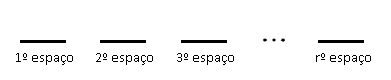
\includegraphics[width=7cm]{C:/Users/Andressa-PC/Desktop/estatistica/esqueleto/imagens/arranjo_demo.png}

\end{figure}

Assim, A(n,r) pode ser considerado a quantidade de maneiras de colocar \textbf{\textit{n}} objetos distintos em \textbf{\textit{r}} espaços.

Supondo primeiramente que o número de objetos é igual ao número de espaços (\textbf{\textit{n}}=\textbf{\textit{r}}), teríamos n objetos para ocupar o primeiro espaço, n-1 para o segundo, n-3 para o terceiro e assim por diante, de forma que ao chegar no último espaço teremos apenas um objeto para escolher.
Logo, pelo princípio fundamental da contagem descrito anteriormente temos
\begin{center}
	$A(n,n)=n\ \ .\ \ (n-1)\ \ .\ \ (n-2)\ \ .\ \ (n-3)\ \ ...\ \ 1$
\end{center}

\noindent 
que é a definição de fatorial, ou seja, o produto de todos os inteiros de \textbf{\textit{n}} até 1 (Niven, 1965). Assim,
\begin{center}
	$A(n,n)=n!$
\end{center}

\noindent 
Por exemplo, 
\begin{center}
	$A(4,4)= 4\ \ .\ \ 3\ \ .\ \ 2\ \ .\ \ 1\ \ =\ \ 4!$
\end{center}
Isso também pode ser aplicado para um A(n,r), ou seja, para o caso em que o número de espaços é menor que o número de objetos. Por exemplo,
\begin{center}
	$A(10,4)= 10\ \ .\ \ 9\ \ .\ \ 8\ \ .\ \ 7$
\end{center}
Generalizando, podemos dizer que
\begin{center}
	$A(n,r)\ \ =\ \ n\ \ .\ \ (n-1)\ \ .\ \ (n-2)\ \ .\ \ (n-3),...,(n-(r-1))$

ou

	$A(n,r)\ \ =\ \ n\ \ .\ \ (n-1)\ \ .\ \ (n-2)\ \ .\ \ (n-3)\ \ ...\ \ (n-r+1)$
\end{center}

\noindent
multiplicando por $\frac{(n-r)!}{(n-r)!}$, podemos reescrever A(n,r) como\\

$A(n,r)\ \ =\ \ n\ \ .\ \ (n-1)\ \ .\ \ (n-2)\ \ .\ \ (n-3)\ \ ...\ \ (n-r+1)\ \ .\ \ \frac{(n-r)!}{(n-r)!}$

\hspace{\parindent}
$=\ \ \frac{n\ \ .\ \ (n-1)\ \ .\ \ (n-2)\ \ .\ \ (n-3)\ \ ...\ \ (n-r+1)\ \ .\ \ (n-r)!}{(n-r)!}$ 

\hspace{\parindent}
$=\ \ \frac{n\ \ .\ \ (n-1)\ \ .\ \ (n-2)\ \ .\ \ (n-3)\ \ ...\ \ (n-r+1)\ \ .\ \ (n-r)\ \ ...\ \ 3\ \ . \ \ 2 \ \ . \ \ 1}{(n-r)!}$ 

\hspace{\parindent}
$=\ \ \frac{n!}{(n-r)!}$\\

\noindent
pois, como descrito anteriormente, sabemos que no fatorial vamos subtraindo uma unidade de n até alcançar o 1

\begin{center}
	$n!\ \ =\ \ n\ \ .\ \ (n-1)\ \ .\ \ (n-2)\ \ .\ \ (n-3)\ \ ...\ \ (n-r+1)\ \ .\ \ (n-r)\ \ ...\ \ 3\ \ . \ \ 2 \ \ . \ \ 1$
\end{center}

\noindent
Dessa forma, chegamos a fórmula de arranjo
\begin{equation}
A(n,r) = \frac{n!}{(n-r)!}
\end{equation}

\noindent
Exemplo 1: Em certo país as placas dos automóveis tem letras, e não números,que as distinguem. Precisamente quatro letras são usadas. Quantas placas podem ser feitas se contamos com um alfabeto de 26 letras? E se não fosse permitido usar letras repetidas em uma placa?

Para a primeira letra da placa teremos 26 opções, para a segunda também teremos 26 opções, e assim por diante. Se há 4 posições possíveis para alocar essas letras, então teremos $26^4$ possibilidades de escolha.

Se não utilizarmos letras repetidas, ficamos com 26.25.24.23 ou  $\frac{26!}{22!}$ possibilidades de escolha\\

\noindent
Exemplo 2: Quantos inteiros entre 100 e 999 inclusivo consiste de dígitos ímpares distintos?

Os dígitos ímpares são 1, 3, 5, 7 e 9, logo n=5. Além disso, os número serão formados por 3 dígitos, logo r=3. Assim podemos dizer que vamos realizar uma permutação de 5 objetos tomados 3 a 3, ou seja, A(5,3).

\begin{center}
	$A(5,3) = \frac{5!}{(5-3)!}= \frac{5!}{2!}=\frac{5.4.3.2!}{2!}=5.4.3=60$
\end{center}




\section*{Combinações}
\addcontentsline{toc}{section}{Combinações}
Uma combinação simples é um subconjunto com k elementos de um conjunto universo com n elementos. É interessante ressaltar a ideia de conjunto pois a ordem dos elementos de um subconjunto não altera sua identidade, ou seja, um subconjunto $\{a, b, c\}$ é o mesmo que $\{c , a, b\}$.

Representado pelo símbolo matemático $\mathrm{C}_k^n$, que significa ``o número de combinações, tomadas $k$ a $k$, que podem se selecionadas de um total de $n$ objetos distintos''.  É esperado que $k \leq n$, visto que estamos calculando o número de maneiras de escolher $k$ objetos de um total $n$.

Sabemos que uma coleção de n objetos pode ser ordenada de $n!$ jeitos. Caso quiséssemos organizar esses $n$ objetos no intervalo de $k$ a $n$ teríamos um arranjo com repetição dado pela fórmula $ \dfrac{n!}{(n - k)!}$ estudada anteriormente. Então se quiséssemos calcular as maneiras de selecionar esses objetos de forma que a ordem deles não importasse, ou seja, uma ordem $\{a, b, c\}$ sendo o mesmo que $\{c , a, b\}$, teríamos então que remover a quantidade de permutações entre esses objetos, dividindo pelo número de formas que eles se arranjam entre si, dessa forma teríamos $\dfrac{\dfrac{n!}{n-k}}{k!}$o que nos induz a fórmula $\dfrac{n!}{k!(n-k)}$.

\subsection*{Questão 1}

\begin{wrapfigure}{l}{0.4\textwidth}
	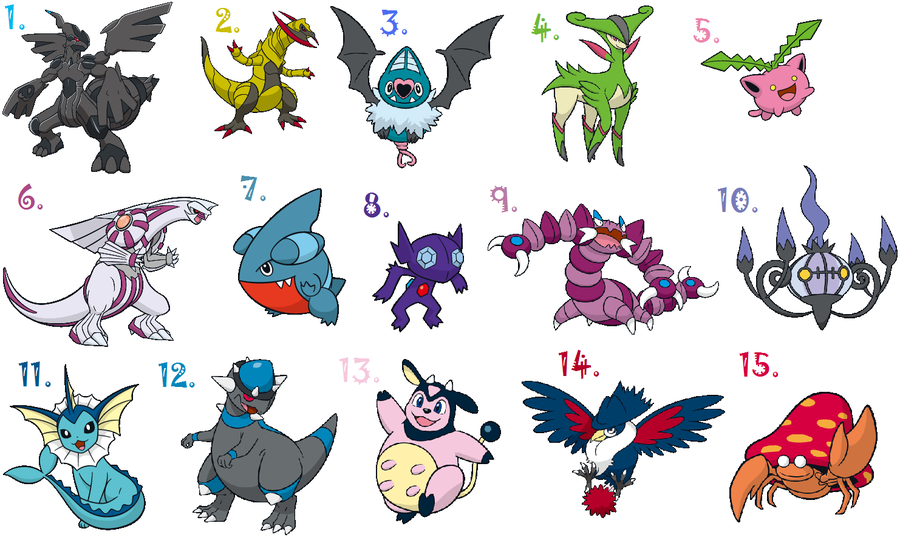
\includegraphics[width=5cm, left]{imagens/pokemon.png}
\end{wrapfigure}

Um treinador pokemon possui a sua disposição 15 pokemons, mas ele só pode carregar 6 pokemons de cada vez, então ele decidiu contar de quantas maneiras diferentes ele poderia escolher um time com 6 dessas criaturinhas.

\subsubsection*{Resolução da questão 1}

Note que o treinador não se atentou aos tipos de pokemons que dispunha, dessa forma ele só quer calcular o número de combinações que formam um time de 6, o que pode ser facilmente calculado pela fórmula mostrada anteriormente: $\dfrac{15!}{6!(15-6)}$, o que resulta em um total de 5005 maneiras de formar times pokemons.

\subsection*{Questão 2}

\begin{wrapfigure}{l}{0.4\textwidth}
	
\includegraphics[width=5cm, left]{imagens/mst.png}
\end{wrapfigure}

(UFSM) A reforma agrária ainda é um ponto crucial para se estabelecer uma melhor distribuição de renda no Brasil. Uma comunidade de sem-terra, após se alojar numa fazenda comprovadamente improdutiva, recebe informação de que o INCRA irá receber uma comissão para negociações. Em assembléia democrática, os sem-terra decidem que tal comissão será composta por um presidente geral, um porta-voz que repassará as notícias à comunidade e aos representantes e um agente que cuidará da parte burocrática das negociações. Além desses com cargos específicos, participarão dessa comissão mais 6 conselheiros que auxiliarão indistintamente em todas as faces da negociação.
Se, dentre toda a comunidade, apenas 15 pessoas forem consideradas aptas aos cargos, o número de comissões distintas que poderão ser formadas com essas 15 pessoas é obtido pelo produto

\subsubsection*{Resolução da questão 2}

Existem os 3 cargos principais para serem preenchidos pelos 15 sem-terra, assim como os 6 cargos restantes de conselheiros, sendo assim, iremos ter 15 pessoas concorrendo aos cargos principais e depois de preencher esses cargos, 12 pessoas estarão concorrendo a conselheiros.

Note que, para a posição dos cargos principais é importante, ou seja, as pessoas a, b e c, por ocuparem cargos diferentes formam novos grupos, então temos que distribuir os 15 sem-terra entre os 3 cargos, tendo então 15 possibilidades de escolha para presidente, 14 para porta-voz e 13 para agente, totalizando $15 \cdot 14 \cdot 13$ arranjos desses cargos.

Para os cargos de conselheiros um grupo contendo as pessoas ``a, b, c, d'' e ``e'' são o mesmo grupo, não importa a ordem de disposição dos sem-terra, dessa forma teríamos uma combinação das 12 pessoas restantes para um grupo de 6, utilizando a fórmula teremos $\dfrac{12!}{6!(12-6)}$ que implica em $11 \cdot 7 \cdot 3 \cdot 2^{2}$.

Contabilizando as possibilidades de conselheiros e cargos principais teremos  $15 \cdot 14 \cdot 13 \cdot 11 \cdot 7 \cdot 3 \cdot 2^{2}$ formas de organizar comissões distintas formadas pelos 15 sem-terra.


\begin{comment}

%Esse postextual só é usado em caso de referências

\postextual

\onecolumn{
	\bibliography{bibliography}
}

\end{comment}

\end{document}
